\documentclass{standalone}
\usepackage{tikz}
\usetikzlibrary{patterns, positioning}


\begin{document}
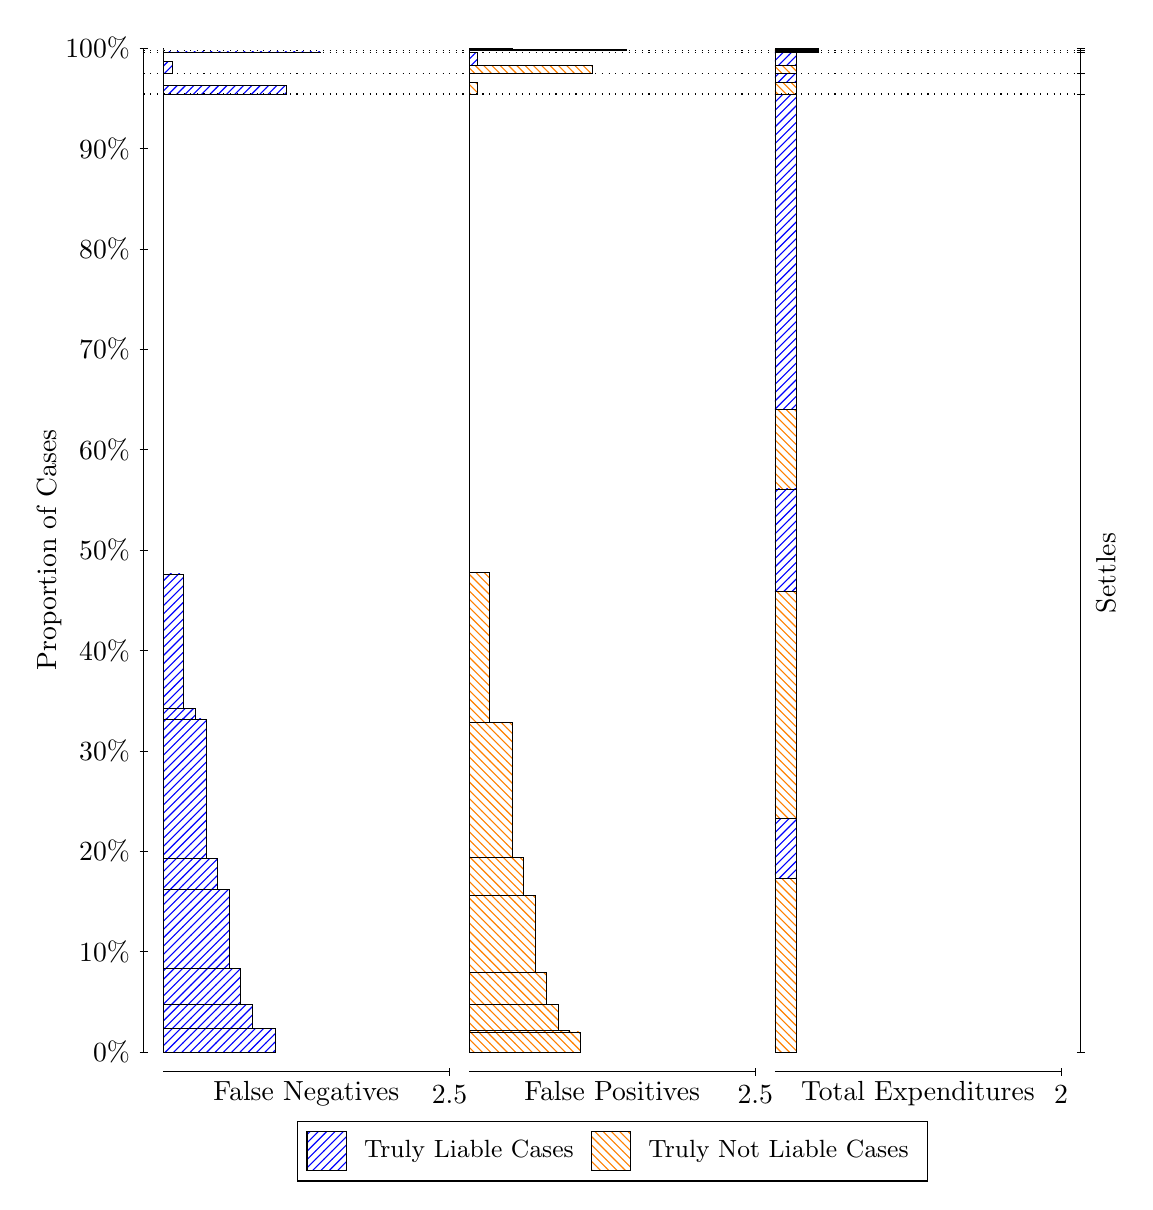
\begin{tikzpicture}
\draw[black, very thin] (1.5,1.75) -- (1.5,14.5);
\node[rotate=90, text=black, anchor=center] at (0.3, 8.125) {Proportion of Cases};
\draw[black, very thin] (1.45,1.75) -- (1.55,1.75);
\node[text=black, anchor=east] at (1.45, 1.75) {0\%};
\draw[black, very thin] (1.45,3.025) -- (1.55,3.025);
\node[text=black, anchor=east] at (1.45, 3.025) {10\%};
\draw[black, very thin] (1.45,4.3) -- (1.55,4.3);
\node[text=black, anchor=east] at (1.45, 4.3) {20\%};
\draw[black, very thin] (1.45,5.575) -- (1.55,5.575);
\node[text=black, anchor=east] at (1.45, 5.575) {30\%};
\draw[black, very thin] (1.45,6.85) -- (1.55,6.85);
\node[text=black, anchor=east] at (1.45, 6.85) {40\%};
\draw[black, very thin] (1.45,8.125) -- (1.55,8.125);
\node[text=black, anchor=east] at (1.45, 8.125) {50\%};
\draw[black, very thin] (1.45,9.4) -- (1.55,9.4);
\node[text=black, anchor=east] at (1.45, 9.4) {60\%};
\draw[black, very thin] (1.45,10.675) -- (1.55,10.675);
\node[text=black, anchor=east] at (1.45, 10.675) {70\%};
\draw[black, very thin] (1.45,11.95) -- (1.55,11.95);
\node[text=black, anchor=east] at (1.45, 11.95) {80\%};
\draw[black, very thin] (1.45,13.225) -- (1.55,13.225);
\node[text=black, anchor=east] at (1.45, 13.225) {90\%};
\draw[black, very thin] (1.45,14.5) -- (1.55,14.5);
\node[text=black, anchor=east] at (1.45, 14.5) {100\%};

\draw[black, very thin] (13.4,1.75) -- (13.4,14.5);
\draw[black, very thin] (13.35,1.75) -- (13.45,1.75);
\node[anchor=west] at (13.35, 1.75) {};
\draw[black, very thin] (13.35,13.916) -- (13.45,13.916);
\node[anchor=west] at (13.35, 13.916) {};
\draw[black, very thin] (13.35,14.174) -- (13.45,14.174);
\node[anchor=west] at (13.35, 14.174) {};
\draw[black, very thin] (13.35,14.442) -- (13.45,14.442);
\node[anchor=west] at (13.35, 14.442) {};
\draw[black, very thin] (13.35,14.47) -- (13.45,14.47);
\node[anchor=west] at (13.35, 14.47) {};
\draw[black, very thin] (13.35,14.5) -- (13.45,14.5);
\node[anchor=west] at (13.35, 14.5) {};

\draw[black, very thin, pattern color=blue, pattern=north east lines] (1.75,1.75) rectangle (3.167,2.0485);
\draw[black, very thin, pattern color=blue, pattern=north east lines] (1.75,2.0485) rectangle (2.8763,2.3578);
\draw[black, very thin, pattern color=blue, pattern=north east lines] (1.75,2.3578) rectangle (2.731,2.8139);
\draw[black, very thin, pattern color=blue, pattern=north east lines] (1.75,2.8139) rectangle (2.5857,3.8171);
\draw[black, very thin, pattern color=blue, pattern=north east lines] (1.75,3.8171) rectangle (2.4403,4.2071);
\draw[black, very thin, pattern color=blue, pattern=north east lines] (1.75,4.2071) rectangle (2.295,5.9811);
\draw[black, very thin, pattern color=blue, pattern=north east lines] (1.75,5.9811) rectangle (2.1497,6.1184);
\draw[black, very thin, pattern color=blue, pattern=north east lines] (1.75,6.1184) rectangle (2.0043,7.8224);
\draw[black, very thin, pattern color=orange, pattern=north west lines] (1.75,7.8224) rectangle (1.75,13.916);
\draw[black, very thin, pattern color=blue, pattern=north east lines] (1.75,13.916) rectangle (3.3123,14.029);
\draw[black, very thin, pattern color=orange, pattern=north west lines] (1.75,14.029) rectangle (1.75,14.174);
\draw[black, very thin, pattern color=blue, pattern=north east lines] (1.75,14.174) rectangle (1.859,14.333);
\draw[black, very thin, pattern color=orange, pattern=north west lines] (1.75,14.333) rectangle (1.75,14.442);
\draw[black, very thin, pattern color=blue, pattern=north east lines] (1.75,14.442) rectangle (3.7483,14.451);
\draw[black, very thin, pattern color=orange, pattern=north west lines] (1.75,14.451) rectangle (1.75,14.47);
\draw[black, very thin, pattern color=orange, pattern=north west lines] (1.75,14.47) rectangle (1.75,14.479);
\draw[black, very thin, pattern color=blue, pattern=north east lines] (1.75,14.479) rectangle (1.75,14.5);
\draw[black, very thin, pattern color=orange, pattern=north west lines] (5.6333,1.75) rectangle (7.0503,2.0044);
\draw[black, very thin, pattern color=orange, pattern=north west lines] (5.6333,2.0044) rectangle (6.905,2.0261);
\draw[black, very thin, pattern color=orange, pattern=north west lines] (5.6333,2.0261) rectangle (6.7597,2.3577);
\draw[black, very thin, pattern color=orange, pattern=north west lines] (5.6333,2.3577) rectangle (6.6143,2.7601);
\draw[black, very thin, pattern color=orange, pattern=north west lines] (5.6333,2.7601) rectangle (6.469,3.736);
\draw[black, very thin, pattern color=orange, pattern=north west lines] (5.6333,3.736) rectangle (6.3237,4.2214);
\draw[black, very thin, pattern color=orange, pattern=north west lines] (5.6333,4.2214) rectangle (6.1783,5.9382);
\draw[black, very thin, pattern color=orange, pattern=north west lines] (5.6333,5.9382) rectangle (5.8877,7.8435);
\draw[black, very thin, pattern color=blue, pattern=north east lines] (5.6333,7.8435) rectangle (5.6333,13.916);
\draw[black, very thin, pattern color=orange, pattern=north west lines] (5.6333,13.916) rectangle (5.7423,14.061);
\draw[black, very thin, pattern color=blue, pattern=north east lines] (5.6333,14.061) rectangle (5.6333,14.174);
\draw[black, very thin, pattern color=orange, pattern=north west lines] (5.6333,14.174) rectangle (7.1957,14.283);
\draw[black, very thin, pattern color=blue, pattern=north east lines] (5.6333,14.283) rectangle (5.7423,14.442);
\draw[black, very thin, pattern color=orange, pattern=north west lines] (5.6333,14.442) rectangle (5.6333,14.461);
\draw[black, very thin, pattern color=blue, pattern=north east lines] (5.6333,14.461) rectangle (5.6333,14.47);
\draw[black, very thin, pattern color=orange, pattern=north west lines] (5.6333,14.47) rectangle (7.6317,14.479);
\draw[black, very thin, pattern color=blue, pattern=north east lines] (5.6333,14.479) rectangle (6.1783,14.5);
\draw[black, very thin, pattern color=orange, pattern=north west lines] (9.5167,1.75) rectangle (9.7892,3.9522);
\draw[black, very thin, pattern color=blue, pattern=north east lines] (9.5167,3.9522) rectangle (9.7892,4.7176);
\draw[black, very thin, pattern color=orange, pattern=north west lines] (9.5167,4.7176) rectangle (9.7892,7.5988);
\draw[black, very thin, pattern color=blue, pattern=north east lines] (9.5167,7.5988) rectangle (9.7892,8.9005);
\draw[black, very thin, pattern color=orange, pattern=north west lines] (9.5167,8.9005) rectangle (9.7892,9.9106);
\draw[black, very thin, pattern color=blue, pattern=north east lines] (9.5167,9.9106) rectangle (9.7892,13.916);
\draw[black, very thin, pattern color=orange, pattern=north west lines] (9.5167,13.916) rectangle (9.7892,14.061);
\draw[black, very thin, pattern color=blue, pattern=north east lines] (9.5167,14.061) rectangle (9.7892,14.174);
\draw[black, very thin, pattern color=orange, pattern=north west lines] (9.5167,14.174) rectangle (9.7892,14.283);
\draw[black, very thin, pattern color=blue, pattern=north east lines] (9.5167,14.283) rectangle (9.7892,14.442);
\draw[black, very thin, pattern color=orange, pattern=north west lines] (9.5167,14.442) rectangle (10.062,14.461);
\draw[black, very thin, pattern color=blue, pattern=north east lines] (9.5167,14.461) rectangle (10.062,14.47);
\draw[black, very thin, pattern color=orange, pattern=north west lines] (9.5167,14.47) rectangle (10.062,14.479);
\draw[black, very thin, pattern color=blue, pattern=north east lines] (9.5167,14.479) rectangle (10.062,14.5);
\draw[black, dotted] (1.5,13.916) -- (13.4,13.916);
\draw[black, dotted] (1.5,14.174) -- (13.4,14.174);
\draw[black, dotted] (1.5,14.442) -- (13.4,14.442);
\draw[black, dotted] (1.5,14.47) -- (13.4,14.47);
\draw[black, very thin] (1.75,1.5) -- (5.3833,1.5);
\node[text=black, anchor=north] at (3.5667, 1.5) {False Negatives};
\draw[black, very thin] (5.3833,1.45) -- (5.3833,1.55);
\node[text=black, anchor=north] at (5.3833, 1.45) {2.5};

\draw[black, very thin] (5.6333,1.5) -- (9.2667,1.5);
\node[text=black, anchor=north] at (7.45, 1.5) {False Positives};
\draw[black, very thin] (9.2667,1.45) -- (9.2667,1.55);
\node[text=black, anchor=north] at (9.2667, 1.45) {2.5};

\draw[black, very thin] (9.5167,1.5) -- (13.15,1.5);
\node[text=black, anchor=north] at (11.333, 1.5) {Total Expenditures};
\draw[black, very thin] (13.15,1.45) -- (13.15,1.55);
\node[text=black, anchor=north] at (13.15, 1.45) {2};

\node[text=black, centered, rotate=90] at (13.72, 7.8329) {Settles};





\draw (7.449999999999999,1.5) node[draw=none] (baseCoordinate) {};
\begin{scope}[align=center]
        \matrix[scale=0.5, draw=black, below=0.5cm of baseCoordinate, nodes={draw}, column sep=0.1cm]{
            \node[rectangle, draw, minimum width=0.5cm, minimum height=0.5cm, pattern color=blue, pattern=north east lines] {}; &
            \node[draw=none, font=\small, text=black] (B) {Truly Liable Cases}; &
            \node[rectangle, draw, minimum width=0.5cm, minimum height=0.5cm, pattern color=orange, pattern=north west lines] {}; &
            \node[draw=none, font=\small, text=black] (B) {Truly Not Liable Cases}; \\
            };
\end{scope}

\end{tikzpicture}
\end{document}